% Your name
\renewcommand{\YRname}{R. Oechslin}

% Your grade/post
\newcommand{\YRgrade}{M2}

% Submission date
\newcommand{\YRdate}{2018.Jun.30}

% Your research theme
\newcommand{\YRtheme}{Haptic Feedback Controller with Palm Pressurization}

% Work plan
\newcommand{\YRplan}{
	\hspace{-4truemm}
	\begin{tabularx}{170truemm}{|p{50truemm}||X|X|X|X|X|X|X|X|X|X|X|X|}
		\hline
		\multicolumn{13}{|c|}{\parbox[c][10truemm][c]{0truemm}{} \large Research theme: \bf \YRtheme} \\
		\hline
		\hline
		\multicolumn{13}{|c|}{\parbox[c][8truemm][c]{0truemm}{} \large \bf --- Research Plan ---} \\
		\hline
		Term \textbackslash Month & 2 & 3 & 4 & 5 & 6 & 7 & 8 & 9 & 10 & 11 & 12 & 1 \\
		\hline
		% For ``Work plan'', do not change above.
		\hline
		Literature review & & & & & & & & & & & & \\
		\shadecells{2-2}
		\hline
		Design PlayStation Controller  & & & & & & & & & & & & \\
		\shadecells{2-3}
		\hline
		Test PlayStation Controller & & & & & & & & & & & & \\
		\shadecells{4-6}
		\hline
		Frequency Response Analysis & & & & & & & & & & & & \\
		\shadecells{5-6}
		\hline
		Design Pilot Controller & & & & & & & & & & & & \\
		\shadecells{4-6}
		\hline
		Test Pilot Controller & & & & & & & & & & & & \\
		\shadecells{6-7}
		\hline
		& & & & & & & & & & & & \\
		%\shadecells{2-10}
		\hline
		Theoretical Analysis & & & & & & & & & & & & \\
		\shadecells{6-7}
		\hline
		Analyze data and compare & & & & & & & & & & & & \\
		\shadecells{7-8}
		\hline
		Write Thesis & & & & & & & & & & & & \\
		\shadecells{8-8}
		\hline
	\end{tabularx}
}

% Main contents of your work
\newcommand{\YRachievement}{
	
	\section{Introduction}
	This report is the continuation of the first two reports about the project "Haptic Feedback Controller with Palm Pressurization". The last report has left off ...
	
	
	\section{Theoretical analysis}
	% I can check with existing papers and take their block diagram
	To come up with a theoretical analysis of the transfer function, a simplifying mechanical schematic has been drawn. This schematic can be seen in figure \ref{fig:mechanical_schematic}.
	\begin{figure}[h!]
		\centering
		\includegraphics[width=0.6\linewidth]{Figs/mechanical_schematic}
		\caption{Simplifying mechanical schematic of the actuation system with the stimulator.}
		\label{fig:mechanical_schematic}
	\end{figure}
	The equations of motion can be formulated with the major parameters defined in the schematic. A full explanation of all parameters can be seen in table \ref{}. The variables with subscript $1$ refer to the first mass element, the carriage in its guideway, whereas variables with subscript $2$ refer to the stimulator, the palm pad. For the motor the subscript $m$ has been used.\\ %TODO make this table
	
	\subsection{Assumptions}
	First of all, it is important to mention that the transfer function is non-linear, due to the motor angle $\theta$ that determines the force that acts on the carriage $c_1$. As an initial approach however, this effect has been neglected . More specifically, it is assumed that $\theta \ll 1$ and $\cos{\theta} \frac{T_m}{L_{CL} } = F_{carr} $ becomes $\frac{T_m}{L_{CL} } \simeq F_{carr} $. Furthermore, there are two types of friction in the system. Once from the interior of the motor and bearings and the carriage in its guideway, and then of the second mass, the stimulator also called the palm pad. These two types of friction can be modeled as visquous damping with coefficients $b_1$ and $b_2$ respectively.\\
	As a first approach, it is assumed that both types of friction can be neglected since the stimulator is not touching the walls of the controller and the carriage in its guideway has been optimally manufactured for low friction.
	
	\subsection{Expected Transfer Functions}
	The system can be cut into two major transfer functions. The block diagram including these two transfer functions is depicted in figure \ref{fig:2tf_block_diagram}. 
	
	\begin{figure}[h!]
		\centering
		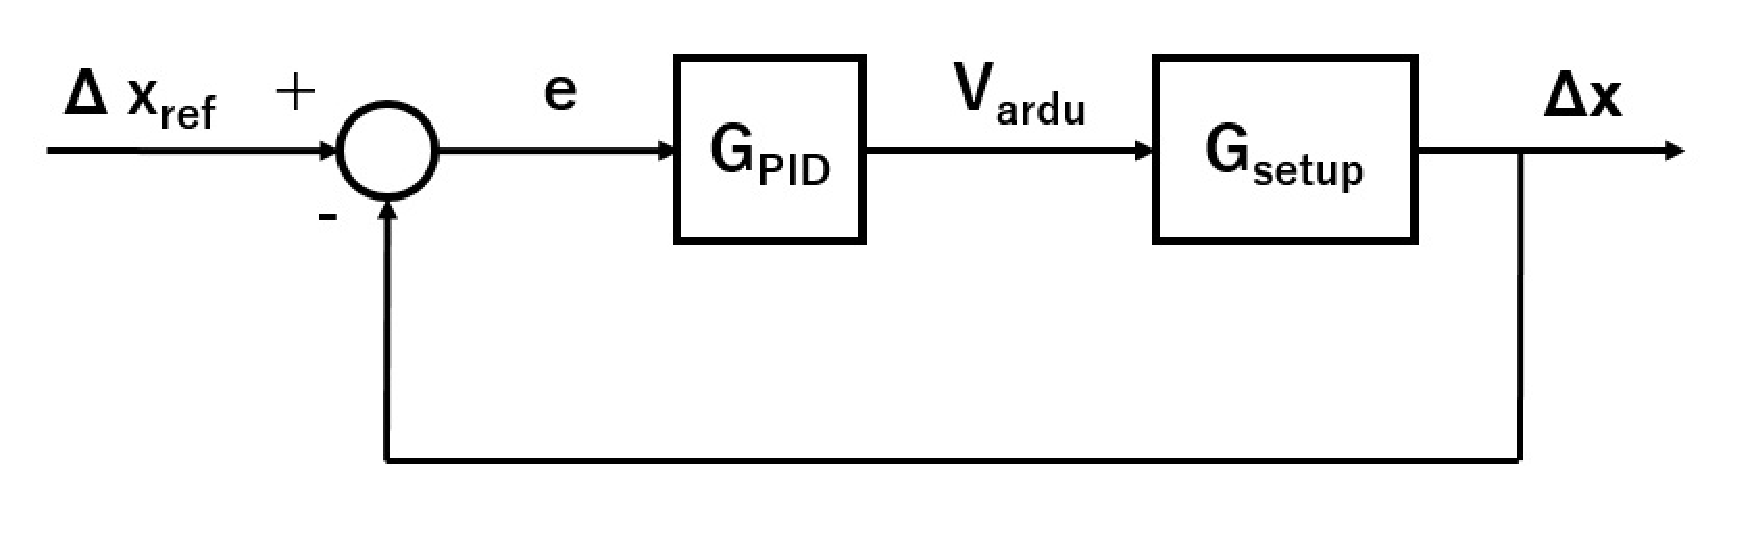
\includegraphics[width=0.6\linewidth]{Figs/2tf_block_diagram}
		\caption{Block diagram with two different transfer functions.}
		\label{fig:2tf_block_diagram}
	\end{figure}
	According to this figure one can obtain a transfer function of the following form:
	\begin{equation}
		F(s) = G_{PID}(s)G_{setup}(s) = \frac{V_{ardu}}{E}\frac{\Delta X}{V_{ardu}} = \frac{\Delta X(s)}{E(s)}
		\label{eq:complete_tf}
	\end{equation}
	Using this form one can calculate the individual transfer functions and finally relate the compression of the springs $\Delta x$ to the compression given as reference $\Delta x_{ref}$.
	\subsubsection{PID Transfer Function}
	The transfer function given by the PID controller is very straight-forward and can be taken out of the books. %FIXME reference here?
	Specific for this case is the multiplication factor $K_{b2V}$ to get from the 8-bit value to the Arduino voltage level. The transfer function is given in equation \ref{eq:tf_pid}. 
	\begin{equation}
		G_{PID} (s) = \frac{V_{ardu}(s)}{E(s)} = K_{b2V} (K_P + \frac{K_I}{s} + K_Ds)
		\label{eq:tf_pid}
	\end{equation}
	
	\subsubsection{Motor Equations}
	The second transfer function relates the motor torque $T_m$ to the Arduino voltage as well as the output $\Delta x$ to $T_m$. Due to the back electromotive force these two parts are related and have to be treated as a whole.
	
	
	The output torque $T_m$ of the motor can be calculated using the sums of all torques and the conversion parameters intrinsic to the motor.\\
	Similar to the setup and analysis in \cite{Junior2016a} the equations of the motor are given as:
	\begin{equation}
		L_a \frac{di_a}{dt} + R_a i_a + K_{emf} \dot{\theta } = V_a
	\end{equation}
	where $L_a$ is the armature inductance, $R_a$ the armature resistance and $i_a$ the armature current of the motor. $K_{emf}$ is the back electromotive force constant also given by the motor. $V_a$ is the armature voltage and $\theta$ is the angle of the motor shaft.\\
	Furthermore, with Newtons law, the sum of all torques must be zero, or:
	\begin{equation}
		J_{T} \ddot{\theta } + b_{1} \dot{\theta} - k_{eq} \Delta x L_{CL} = T_m = K_{\tau} i_a
		\label{eq:torques}
	\end{equation}
	In equation \ref{eq:torques} the parameter $J_{T}$ stands for the total equivalent inertia of the motor and the clamping link, $b_{1}$ is the viscous coefficient used for modeling friction in the motor and $c_1$ and $K_{\tau}$ is the proportional current torque gain constant. The moment of inertia can either be calculated as the sum of all inertias seen by the motor shaft, or measured in a simple test.\\ %TODO state what method I used, maybe compare both?
	Finally, there is also the gain of the amplifier in voltage mode, which converts the voltage of the Arduino into the voltage applied to the motors. This gain is $K_{ampl} = 10$Volt/Volt. To this voltage an offset voltage of $V_{offset} = -20$V is added.\\
	The total inertia of the system is determined by the inertia of the rotor $J_m$, the gear inertia $J_g$, the inertia of the clamp link $J_{CL}$ as well as the inertia of the carriage assembly with mass $m_1$. The last one can be found by simplifying the load to a point mass at distance of the clamp link length $L_{CL}$, which is given by $J_{carr} = m_1 L_{CL}^2$.
	The gear box increases the inertia seen by the motor shaft by the square of its ratio $R$:
	\begin{equation}
		J_{load,\ motor\ side} = R^2 J_{load}
	\end{equation}
	%TODO do I need to take into account the rotor inertia J_m and the gear inertia J_g?
	We have therefore a total inertia of:
	\begin{equation}
		J_T = J_m + J_g + n^2 J_{CL} + n_2^2 m_1 L_{CL}^2
	\end{equation}
	where $J_{CL}$ can be calculated by approximating it as a cantilever with an off-center axis of distance $l$: %Source: http://www.orientalmotor.com/technology/motor-sizing-calculations.html
	%TODO put reference and maybe picture
	
	\begin{equation}
		J_{CL} = \frac{1}{12}m_{CL}(A^2 + B^2 + 12l^2)
	\end{equation}
	where $A$ and $B$ are the width and length respectively.\\
	$n_2^2$ is the equivalent reduction ratio at the point mass $m_1$ taking into account the lever of $L_{CL}$. %TODO how to calculate this
	
	The conversion between the angle $\theta$ and the distance $x$ can be found by assuming that the horizontal displacement of the carriage is given by $L_{CL} sin(\theta) = x$. For small angles of $\theta$ the Taylor expansion gives:
	\begin{equation}
		L_{CL} \theta \simeq x_1
		\label{eq:assum}
	\end{equation} 
	
	The output $\Delta x$ is the compression of the springs and is given by $\Delta x = x_2 - x_1$. For finding $x_2$ the equation of motion given by Newtons law has to be considered.
	
	\begin{equation}
		m_2 \ddot{x}_2 = -k_{eq} (x_2 - x_1) - b_2 \dot{x}_2
		\label{eq:mov_stimul}
	\end{equation}
	Analogously, $b_2$ is the friction coefficient. Using the Laplace transform and equation \ref{eq:mov_stimul} one finds the expression of $x_2$:
	
	\begin{equation}
		X_2 = \frac{k_{eq}}{s^2 m_2 + b_2 s + k_{eq}} X_1
		\label{eq:mov_carr_find_A}
	\end{equation}
	
	\subsubsection{Motor and Spring Transfer Function}
	Combining all the equations one can find the final block diagram, which can be seen in figure \ref{fig:block_diagram}
	\begin{figure}[h!]
		\centering
		\includegraphics[width=0.6\linewidth]{Figs/block_diagram}
		\caption{Complete block diagram relating the output $\Delta x$ to the input $\Delta X_{ref}$.}
		\label{fig:block_diagram}
	\end{figure}


	From this diagram and the equations mentioned above, one can obtain the transfer functions that relate the output $x$ and input $x_{ref}$ as introduced in equation \ref{eq:complete_tf},
	where $X(s)$ and $X_{ref}(s)$ are the Laplace transforms of the output and input functions respectively. \\
	It is thus possible to study the frequency response by simulating the this setup with the assumptions mentioned earlier.
	
	
	% in [amar] p 32 we find coefficients for skin properties, stiffness and damping
	
	
	% the weight m_{CL} is roughly 19 grams, but this has to be confirmed!
	%m_{carr} is roughly 30 grams, but this also has to be confirmed!
	
	%FIXME probably obsolte:
	%$G_{setup}(s)$ can be calculated with the known parameters and a first assumption of negligible viscous friction. This sets external torques $T_{ext}$ to zero.\\
	%Combining all these equations one can find the transfer function of the motor stated in equation \ref{eq:tf_motor}
	
	%\begin{equation}
	%G_{motor} (s) = \frac{\theta(s)}{V_{ardu}(s)} = \frac{K_{ampl} K_{\tau}}{(L_a s + R_a)(J_T s^2 + b_m s) + K_{\tau} K_{emf} s}
	%\label{eq:tf_motor}
	%\end{equation}
	%In fact, one can find an intermediary transfer function $T_1$ such that $\frac{X_1(s)}{\theta(s)} = T_1(s)$. With the expression of $X_2 = A X_1$ one can find the coefficient for the compression: $\Delta X = X_2 - X_1 = T_1 (A-1) \theta$ which is used to simplify the expression later in this analysis.\\
	%\begin{equation}
	%m_1 \ddot{x}_1 = F_{carr} + k_{eq} (x_2 - x_1) - b_1 \dot{x}_1
	%\label{eq:mov_carr}
	%\end{equation}
	
	%Replacing the force $F_{carr}$ in equation \ref{eq:mov_stimul} by $\frac{T_m}{L_{CL}}$ and using equation \ref{eq:torques} and the Laplace transform yields the following expression:
	
	%\begin{equation}
	%\frac{X_1}{\theta} = T_1 = \frac{s^4 J_T m_2 + s^3 (J_T b_2 + m_2 b_m) + s^2 (J_T k_{eq} + b_m b_2) + s b_m k_{eq}}{[s^4 m_1 m_2 + s^3(m_1 b_2 + m_2 b_1) + s^2 ((m_1 + m_2) k_{eq} + b_1 b_2) + s k_{eq} (b_1 + b_2)] L_{CL}}
	%\label{eq:mov_stimul_find_T1}
	%\end{equation}
	
	%Thus one can write the complete expression for $\frac{\Delta X}{\theta}$ as:
	
	%\begin{equation}
	%\begin{split}
	%	\frac{\Delta X(s)}{\theta (s)} = \\
	%	-\frac{(s^4 J_T m_2 + s^3 (J_T b_2 + m_2 b_m) + s^2 (J_T k_{eq} + b_m b_2) + s b_m k_{eq})(s^2 m_2 + b_2 s)}{[s^4 m_1 m_2 + s^3(m_1 b_2 + m_2 b_1) + s^2 ((m_1 + m_2) k_{eq} + b_1 b_2) + s k_{eq} (b_1 + b_2)] L_{CL}(s^2 m_2 + b_2s + k_{eq})}
	%\end{split}
	%\label{eq:tf_mass_spring}
	%\end{equation}
		
	
	\section{Discussion}
	asdfdf

	\section{Conclusion}
	asdf
	
	\section{Outlook}
	faaafaa adsf
	

	
	%�����܂�
}


